\subsection{Tous ensemble}

Toutes les équipes dans l'entreprise travaillent dans un rythme Agile, et chaque équipe choisi l'implémentation qui le convient le plus.

D'un façon global, Bonitasoft travail avec le framework de la figure \ref{frame_safe}

\begin{figure}[!ht]
\centering
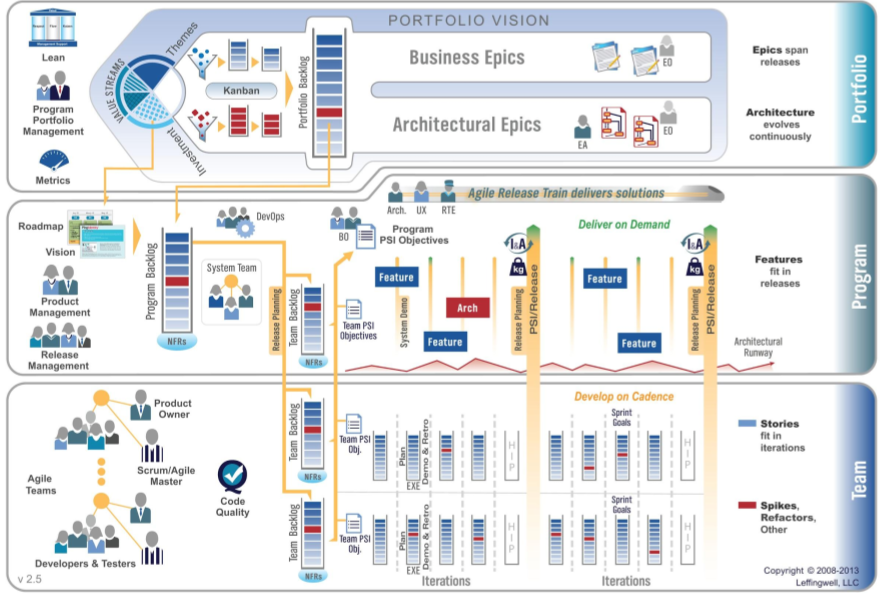
\includegraphics[width=\textwidth,keepaspectratio]{safe_framework.png}
\caption{Cadre de Travail \cite{safe}}
\label{frame_safe}
\end{figure}

Nous voyons dans la partie supérieur que la vision et les fonctionnalités et l'architecture de haut niveau sont définis dans le comité produit, le CEO.
Au milieu, le portfolio est traité et organisé par le Product Manager et à la fin il est développer par le team avec un Product Owner et le Scrum Mater qui dirigent et QA qui assure la qualité du code.
